% Engineering Methods

\documentclass[11pt ,english,a4paper]{article}

\usepackage[english]{babel}
\usepackage[IL2]{fontenc}
\usepackage[utf8]{inputenc}
\usepackage{graphicx}
\usepackage{url}
\usepackage{hyperref}
\usepackage{times}
\usepackage{setspace}

\setstretch{1.5}
\pagestyle{headings}

\title{Efficiency comparative analysis of techniques in misinformation detection in healthcare data\thanks{Semestral project in subject Engineering Methods, ac. year 2023/24, guidance: MSc. Mirwais Ahmadzai}}

\author{Alžbeta Žiarovská\\[2pt]
	{\small Slovak University of Technology in Bratislava}\\
	{\small Faculty of Informatics and Information Technologies}\\
	{\small \texttt{xziarovska@stuba.sk}}
	}

\date{\small 26. september 2023}



\begin{document}

\maketitle
\newpage

\begin{abstract}
\ldots
\end{abstract}
\newpage

\section{Introduction}\label{intro}

In this article I am going to discuss the current situation regarding spread of misinformation in the medical field. This topic is very important in the aftermath of the global COVID-19 pandemic. More specifically I am going to make an analysis and comparison of different misinformation detection methods and their efficiency. During the pandemic we have seen a great rise of misinformation on the Internet, which provide danger to our society or even lives. \cite{war18dr} The main problem in my perception is, that because of the easily accessible information on the Internet, people have lost the ability to differentiate between true and false information and make a conclusion of what they read online by themselves. \cite{ahm23impact} The daily use of social media can increase fear and anxiety and ultimately lead to the delay of diagnosis and receiving the effective healthcare. \cite{wa19sys} The paradox is, that the machines might actually be the solution, as I am going to discuss various methods to recognize misinformation using technology. \cite{chap22unmask}

I am going to focus on comparing fact-checking and machine learning models as s way to find the medical misinformation. The fact-checking can be done manually or automatically which I am going to introduce more deeply in Section \ref{tech:fact}.\cite{bar21health} The other side I am going to take a closer look at are machine learning techniques including Naïve Bayes, Support Vector Machine and BERT-based model called Disease Myth Buster.\cite{bar21health}\cite{chap22unmask} I want to introduce these techniques and compare their efficiency in order to establish which one is the most suitable for a specific situation in healthcare.

In the first Section \ref{ter} I am giving a quick introduction into the terminology used later in the article, so it is easily understandable and could easily be found if necessary. In the Section \ref{mih} I describe the term misinformation, how it differs from disinformation \cite{lazer18science}. Also I am going to give a brief summary of historical development of misinformation spread. \cite{pos18short} It is important as well to mention affect that medical fake news might have on our lives, which I would like to address as well. \cite{who22infodemics} In the last one of the main sections, in Section \ref{tech}, I am taking a closer look at some of the methods used for misinformation recognition. I going to introduce them in a way, that would be easily understandable for all readers and state some of their outputs, so I can compare their effectiveness and possible impact in the future in Conclusion. \ref{conclusion}

\section{Terminology}\label{ter}

\paragraph{Natural language processing} (NLP) is a way for programs to understand language used by humans on daily basis by using various algorithms an limitations. It was originally closely related to information retrieval from written documents, however, over the time, their paths have divided and they no longer have such a vast crossing. \cite{nad11natural}\cite{lid01natural}

\paragraph{Term frequency–inverse document frequency} (TF-IDF) represents a numeric value of how relevant is the specific word for the document in the set of documents. This technique finds its application both in text mining and information retrieval. \cite{chr16tfidf}  

\paragraph{Transfer learning} is a concept of dedicating a new and unusual task where already known knowledge and tools are used for its solution. It is a part of the machine learning, where source tasks are being relocated in order to satisfactorily complete the given task. \cite{chap22unmask}\cite{tor10transfer}

\section{Misinformation in healthcare}\label{mih}

\paragraph{Difference between misinformation and disinformation}
\paragraph{Historical development of concept of misinformation}

\paragraph{General Misinformation}

\paragraph{Health care misinformation}
\paragraph{Societal context}


\section{Misinformation recognition techniques} \label{tech}

\subsection{Fact-checking technique} \label{tech:fact}

\subsubsection{Manual fact-checking}\label{tech:fact:man}

\subsubsection{Automatic fact-checking}\label{tech:fact:auto}

\subsection{Machine learning technique} \label{tech:mach}

\paragraph{Definition}

\paragraph{Text processing}

\subsubsection{Naïve Bayes}

\subsubsection{Support vector machine}

\subsubsection{Disease Myth Buster}

\paragraph{Ethics and sustainability}

\section{Conclusion}\label{conclusion}

Je nejaké riešenie a aké?
Je vaše riešenie podobné iným (hoci aj z inej oblasti a len v z určitého hľadiska)?
O čom je článok, k čomu ste ním prispeli a čo zostáva otvorené?

Z obr.~\ref{f:rozhod} je všetko jasné. 

\begin{figure*}[tbh]
\centering
%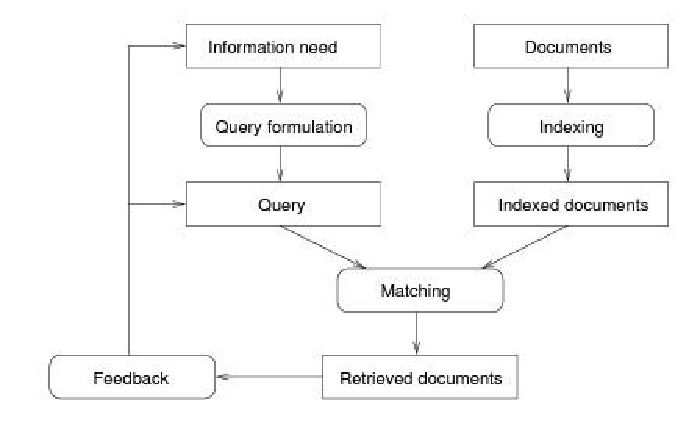
\includegraphics[scale=1.0]{irprocess.pdf}
Aj text môže byť prezentovaný ako obrázok. Stane sa z neho označný plávajúci objekt. Po vytvorení diagramu zrušte znak \texttt{\%} pred príkazom \verb|\includegraphics| označte tento riadok ako komentár (tiež pomocou znaku \texttt{\%}).
\caption{Rozhodujuci argument.}
\label{f:rozhod}
\end{figure*}



\section{Iná časť} \label{ina}

Základným problémom je teda\ldots{} Najprv sa pozrieme na nejaké vysvetlenie (časť~\ref{ina:nejake}), a potom na ešte nejaké (časť~\ref{ina:nejake}).\footnote{Niekedy môžete potrebovať aj poznámku pod čiarou.}

Môže sa zdať, že problém vlastne nejestvuje\cite{bar21health}, ale bolo dokázané, že to tak nie je~\cite{bar21health}. Napriek tomu, aj dnes na webe narazíme na všelijaké pochybné názory\cite{bar21health}. Dôležité veci možno \emph{zdôrazniť kurzívou}.

\section{Ďaľšia časť}
Toto je ďalšia časť, v ktorej idem urobiť odsek.

Toto je odsek. haha.

\subsection{Nejaké vysvetlenie} \label{ina:nejake}

Niekedy treba uviesť zoznam:

\begin{itemize}
\item jedna vec
\item druhá vec
	\begin{itemize}
	\item x
	\item y
	\end{itemize}
\end{itemize}

Ten istý zoznam, len číslovaný:

\begin{enumerate}
\item jedna vec
\item druhá vec
	\begin{enumerate}
	\item x
	\item y
	\end{enumerate}
\end{enumerate}


\subsection{Ešte nejaké vysvetlenie} \label{ina:este}

\paragraph{Veľmi dôležitá poznámka.}
Niekedy je potrebné nadpisom označiť odsek. Text pokračuje hneď za nadpisom.



\section{Dôležitá časť} \label{dolezita}




\section{Ešte dôležitejšia časť} \label{dolezitejsia}




\section{Záver} \label{zaver} % prípadne iný variant názvu



%\acknowledgement{Ak niekomu chcete poďakovať\ldots}


% týmto sa generuje zoznam literatúry z obsahu súboru literatura.bib podľa toho, na čo sa v článku odkazujete
\bibliography{literatura}
\bibliographystyle{alpha} % prípadne alpha, abbrv alebo hociktorý iný
\end{document}
